\section{Perturbation and Gradient-based methods}
The goal of gradient based attribution methods is to estimate the attribution maps $A^c=\{A_i^c\}^N_{i=1}\in \mathbb{R}^N$.
The attribution map $A^c$ captures the importance of each input feature for a specific output class c and has the
same size N as the input.

\subsection{Notaion}
\begin{itemize}
    \item An N dimensional input $\bm{x}=\{x_i\}_{i=1}^N \in \mathbb{R}^N$
    \item A C-dimensional output $S(\bm{x})=\{S_c\}_{c=1}^C \in \mathbb{R}^C$
    \item $S_c(\bm{x})$ represents the network's score function. $S$ can be either a class score or soft-max probability.
\end{itemize}

\subsection{Perturbation-based methods - Occlusion}
Perturbation-based methods directly compute the attribution of an input feature (or set of features) by removing, masking or altering them, and running a forward pass on the new input, measuring the difference with the original output.
The famous occlusion method was presented by \cite{DBLP:conf/eccv/ZeilerF14}. \\
In details each feature $x_i$ (or a set/window of feature for images) is replaced at the time with a zero baseline and the effect of this perturbation is measured 
on the target output:
\begin{equation*}
    A^c = S_c(\bm{x})-S_c(x_{[x_i=0]}) \quad for\; i = 1, \ldots, N
\end{equation*}
where $x_{[x_i=0]}$ indicates a sample $x\in\mathbb{R}^N$ whose ith component component has been replaced with 0.\\

While perturbation-based methods allow a direct estimation of the marginal effect of a feature, they tend to be \textbf{very slow as the number of features to test grows}.\\

\subsection{Gradient-based methods}
\begin{itemize}
    \item Attribution scores are obtained calculating the gradient of the outputs with respect to the extracted features or the input. 
    \item Generally, the gradients are noisy, leading to attribution maps that may show contributions
    from irrelevant features. Various alterations to the gradient-based approach have been
    proposed to handle the challenge of noise in attribution maps
    \item Differently from the backpropagation algorithm used for training, to obtain the saliency
    map what is backpropagated is not the classification error, or loss, but directly the
    classification probability for a given class.
\end{itemize}

\subsubsection{Gradients in the linear case}
We considere a linear model with N+1 parameters $\theta$ and $N$ input features
\begin{equation*}
    y=\theta_0+\sum_{i=1}^N \theta_i x_i+\epsilon = \bm{\theta}^T \bm{x} + \epsilon
\end{equation*}
The partial derivative of the output y with respect to the input $\bm{x}$ results in model parameters $\theta$ which represent contributions of input features.
Thus for the linear case, as seen in previous lessons, model parameters serve as feature attributions.

\subsubsection{Vanilla gradient or Saliency maps}
Introduced by \cite{DBLP:journals/corr/SimonyanVZ13} it's one of the first attribution approaches. It simply calculates the gradient of the class score of interest with respect to the input.
\begin{equation*}
    A^c(x) = |\frac{\partial S_c(x)}{\partial x}| 
\end{equation*}

Algorithm steps:
\begin{enumerate}
    \item Perform a forward pass of the image of interest
    \item Compute the gradient of class score of interest with respect to the input
    \item Visualize the gradients in absolute value
\end{enumerate}

N.B $S_c$ is a nonlinear function of the input x and thus, in contrast to the linear case, the model parameters no more represent feature attributions. It has been shown that saliency maps represent the first-order approximation of the attributions.\\

There is some ambiguity on how to perform a backward pass of the gradients. Non linear units such as ReLU "remove" the sign, so when doing backpass it is not possible
to know whether to assign a positive or negative activation.\\

\textbf{Backpass procedure:}\\
Given the input $x$, during the forward pass, each CNN layer $l$ returns a feature activation map $f^l$ till the last layer $L$.

During the backpass, starting from $f^L$ it is possible to generate the backpropagation map $R^L$ by zeroing all the neuron activations except the one to be backpropagated (the one related to the
target class). This procedure allows to reconstruct the input image $x$ showing the part of the
input image that is most strongly activating this neuron.\\

Each $R^l$ presents an intermediate step in the calculation of the Saliency, for the intermediate
layer $l$. When reaching the CNN input layer, the reconstruction $R^1$ will have the same size of the input $x$.\\

\textbf{Backpass through convolutional layers:}\\
Starting from the convolutional layers, the respective activation in the forward pass can be expressed as: $f_{l+1}=f_l \circledast K_l$, where $K_l$ is a convolutional kernel. The gradient with respect to the output feature map $R^l$, for layer $l$ is then:
\begin{equation*}
    R^l = \frac{\partial R^{L}}{\partial f_l}=\frac{\partial R^{L}}{\partial f_{l+1}}\circledast \hat{K}_l
\end{equation*}
Where $\hat{K}_l$ is the flipped kernel of $K_l$ and $f$ is s the visualized neuron activity.\\
The convolution with the flipped kernel exactly corresponds to computing the $l^{th}$ layer reconstruction $R^l$\\

\textbf{Backpass through ReLU function:}\\
The ReLU is a piece-wise linear function that is defined to be zero for all negative values of the
node input and one otherwise, thus keeping unchanged the positive input values while annihilating
the negative ones.\\
\textbf{i.e.} When the activation of a neuron is zero we do not know which value to backpropagate.

During the forward pass it can be defined as $f_{l+1}(x)=ReLU(f_l)=\max(f_l, 0)$.

The respective backpropagation computes the gradient of $R^l$ with respect to the ReLU layer $l$ as:
\begin{equation*}
    R^l=\frac{\partial R^{L}}{\partial f_l}=\frac{\partial R^{L}}{\partial f_{l+1}}\cdot (f_l>0)=R^{l+1}\cdot (f_l>0)
\end{equation*}
$(f_l>0)$ defines which gradients are backpropagated and is also known as sign operator.\\
In summary it passes gradient to a previous layer only if the original input was positive (the neurons are not dead).
\newpage
Example:
\begin{figure}[H]
    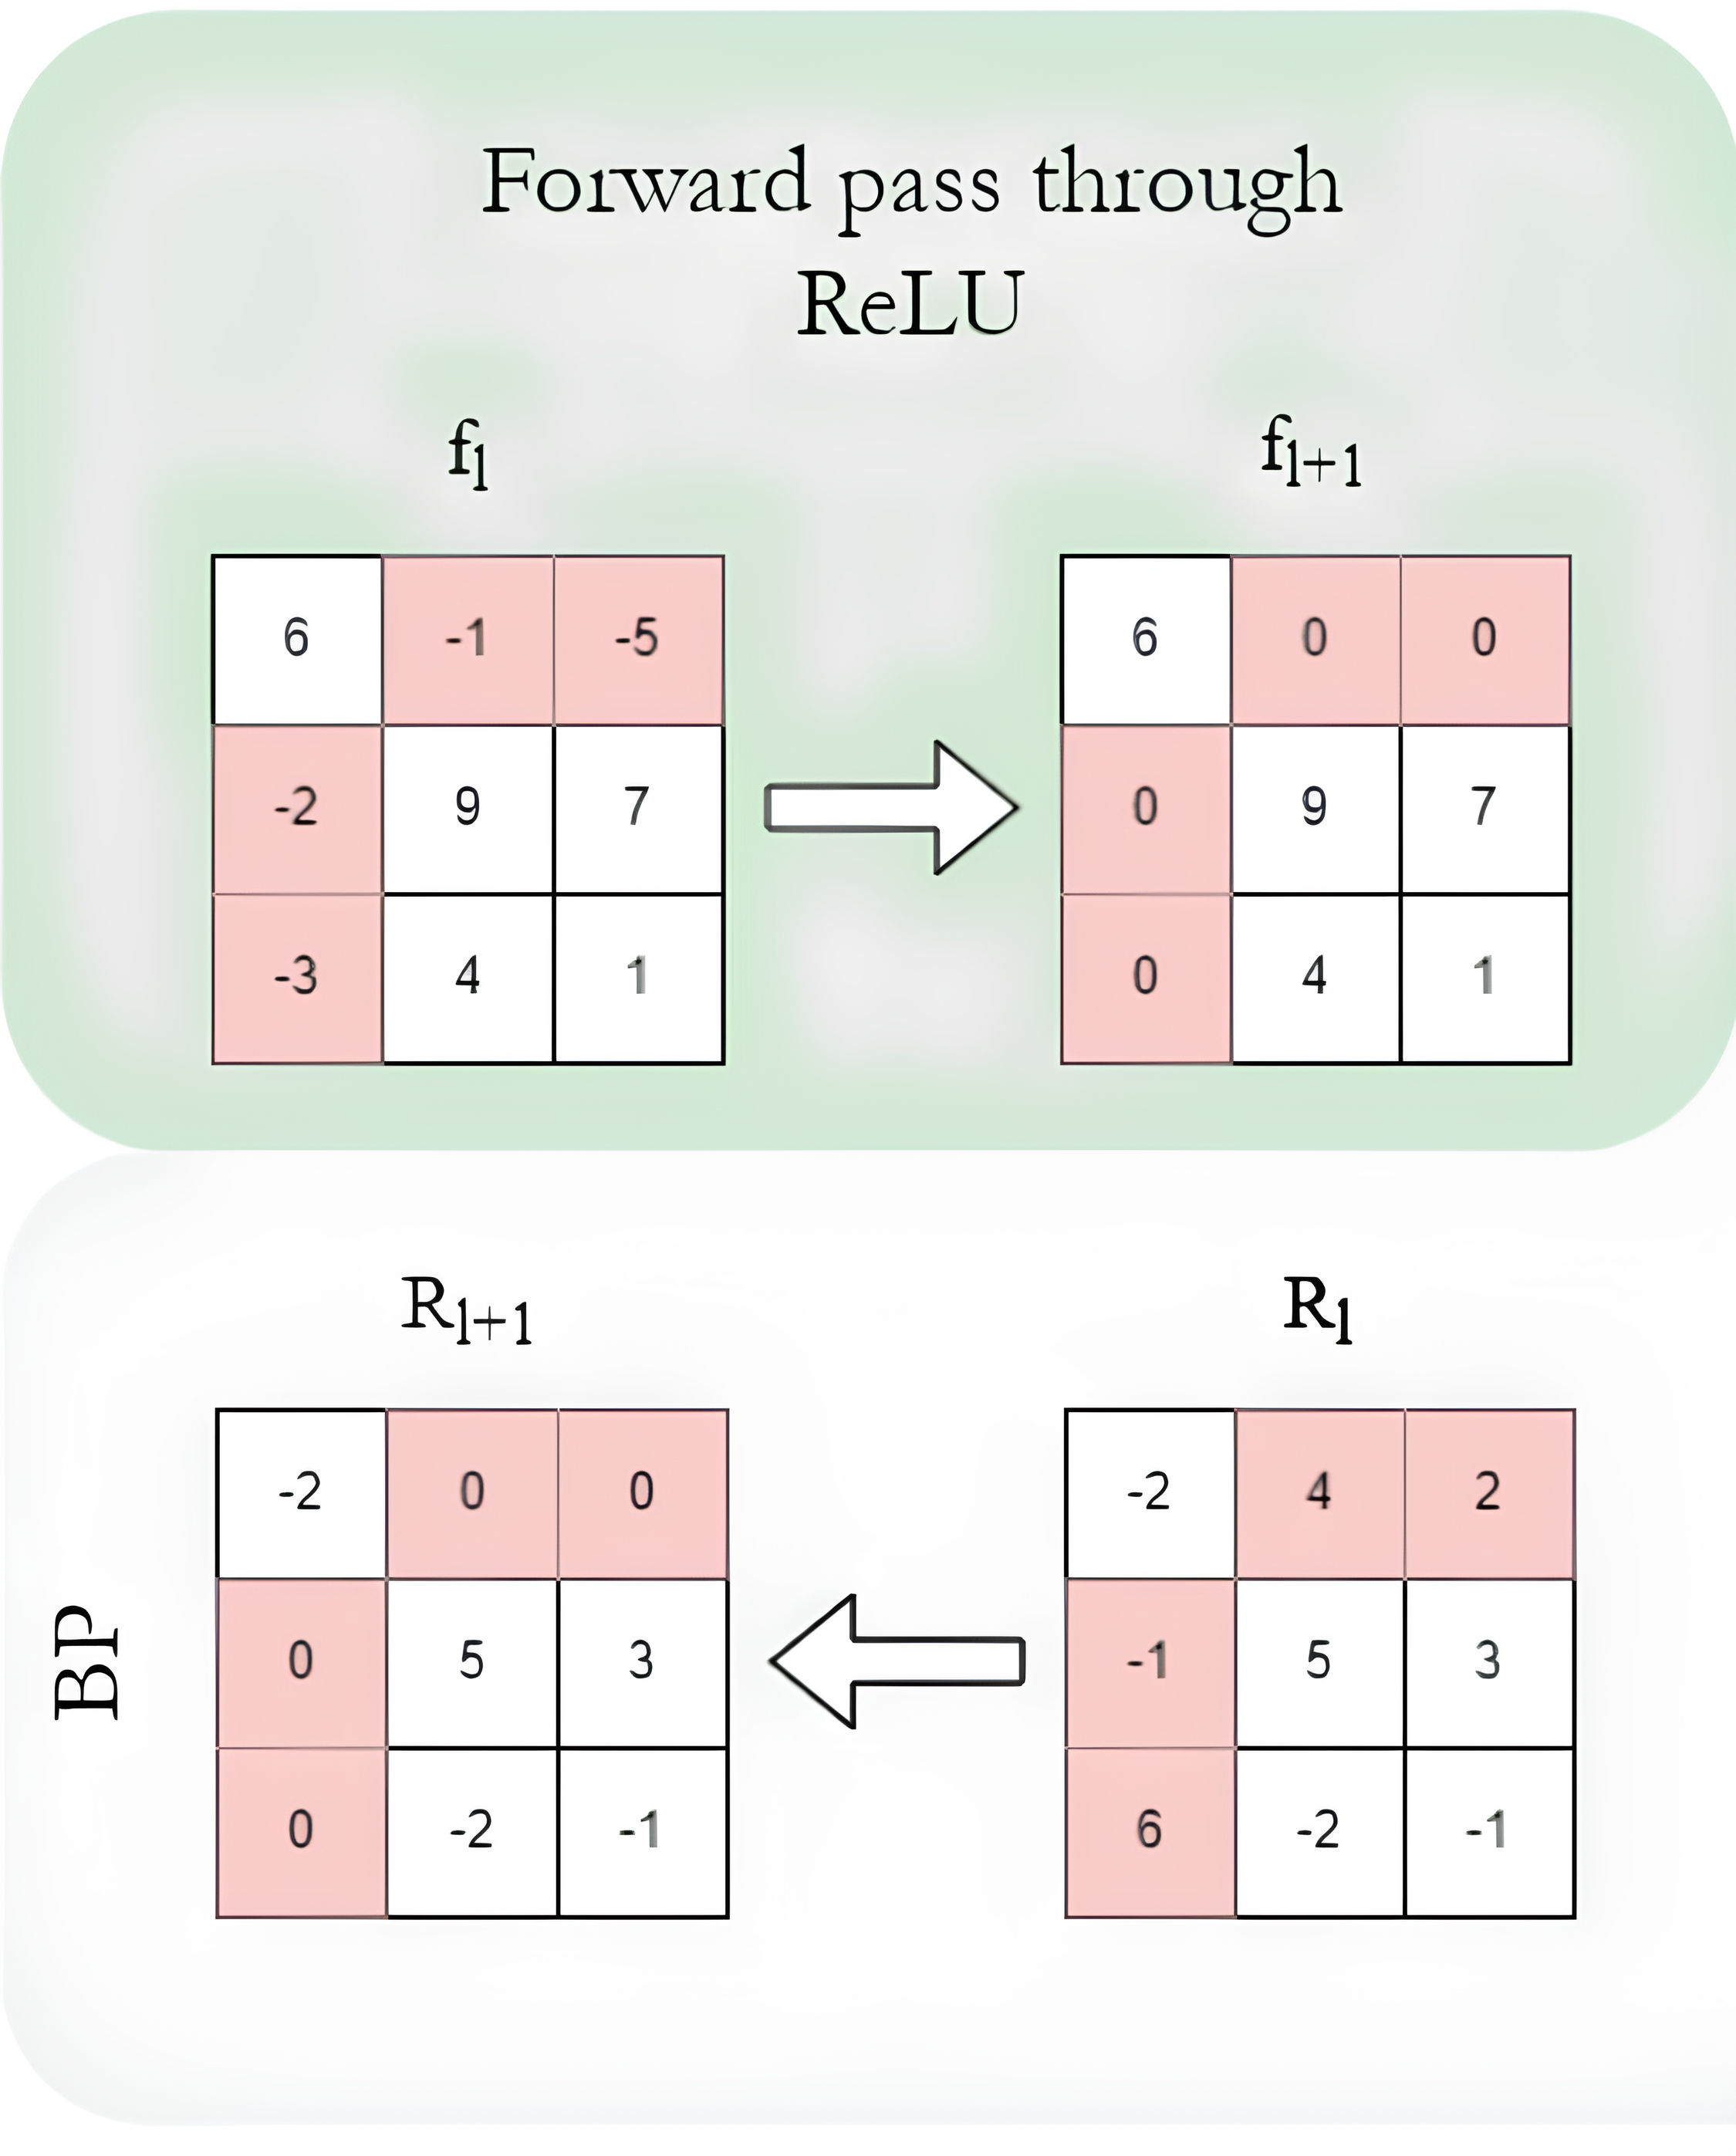
\includegraphics[width=0.3\textwidth]{img/backprop_relu.png}
    \centering
\end{figure}

\subsubsection{DeconvNet}
DeconvNet by \cite{DBLP:conf/eccv/ZeilerF14} is almost identical to Vanilla Gradient but makes a
different choice for backpropagating the gradient through ReLU layer $l$
\begin{equation*}
    R^l=\frac{\partial R^{L}}{\partial f_l}=\frac{\partial R^{L}}{\partial f_{l+1}}\cdot (R^{l+1}>0)=R^{l+1}\cdot (R^{l+1}>0)
\end{equation*}

\begin{minipage}{0.55\textwidth}
    \begin{figure}[H]
        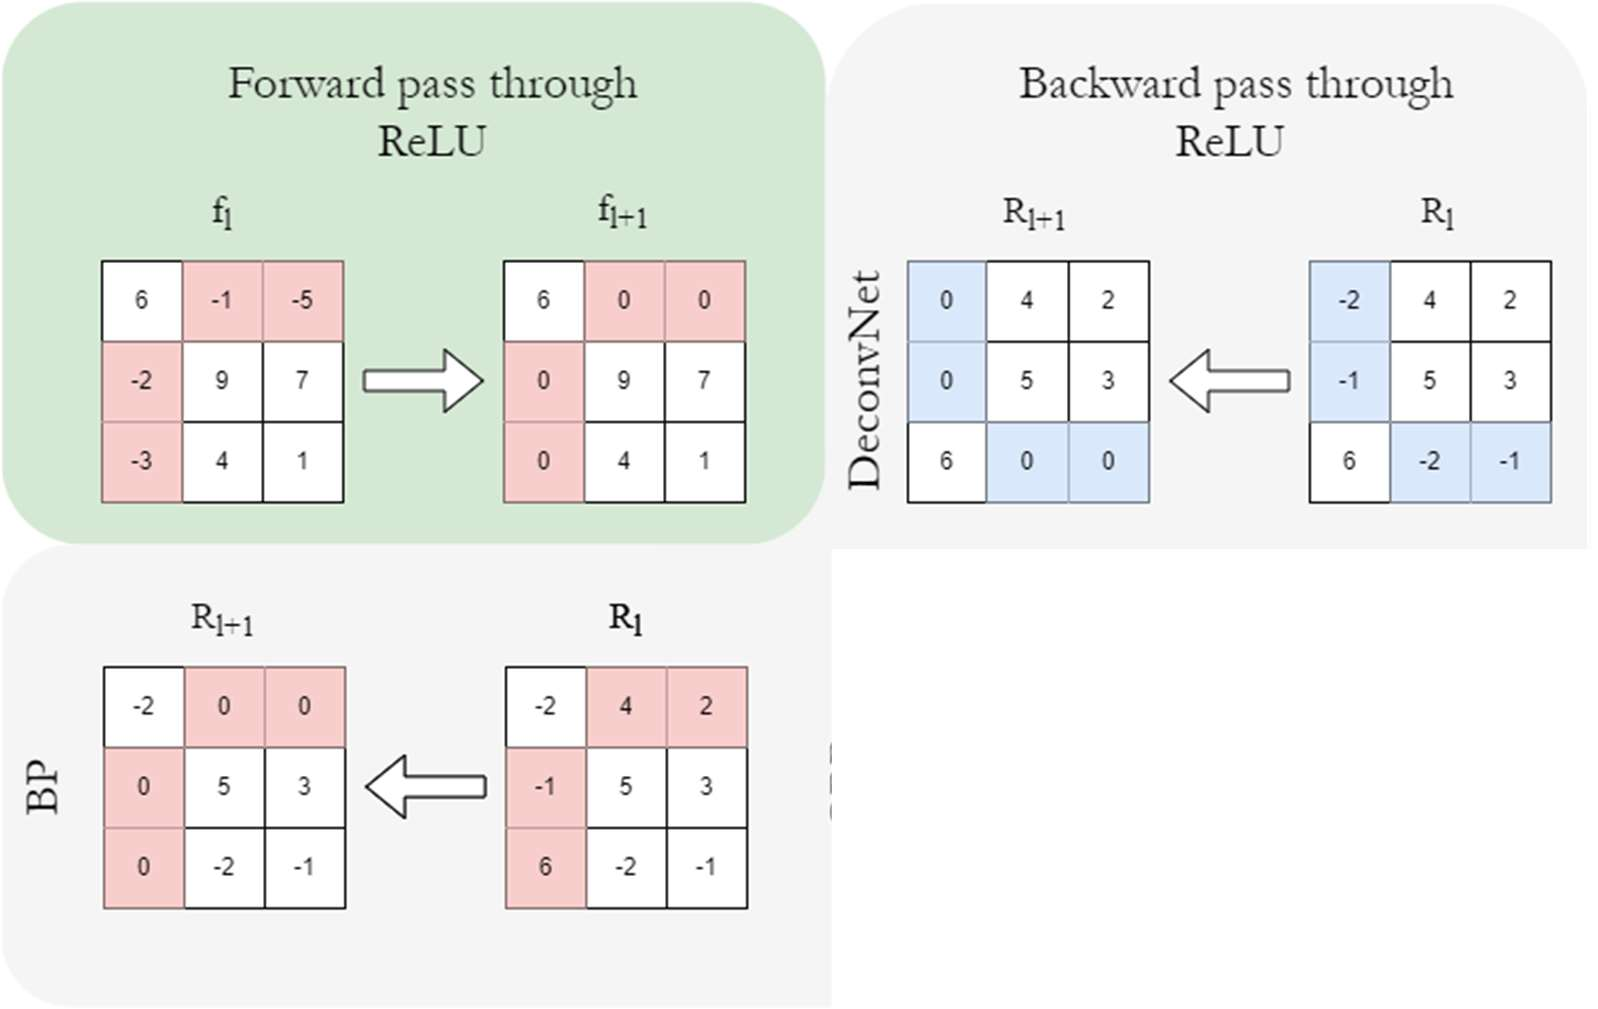
\includegraphics[width=\textwidth]{img/DeconvNet.png}
        \centering
    \end{figure}    
\end{minipage}
\hfill
\begin{minipage}{0.4\textwidth}
    \underline{Difference with saliency:} the sign indicator is based on the output reconstruction $R^{l+1}$ of the precedent layer and not on the input activation $f_l$ to the layer.
    \textbf{This allows only positive error signals to be backpropagated through the net} to obtain the final saliency map.
    When backpassing from layer $l+1$ to layer $l$, DeconvNet “remembers” which of the activations in layer $l+1$ were set to zero in the forward pass and sets them to zero in layer $l$. Activations with a
    negative value in layer $l+1$ are set to zero in layer $l$.
\end{minipage}

\subsubsection{Guided backpropagation}
Presented by \cite{DBLP:journals/corr/SpringenbergDBR14} GBP combines DeconvNet and Saliency, leading to more
focused heatmaps.\\
The difference again is on the backpass through the ReLU layer $l$ which for GBP is defined as:
\begin{equation*}
    R^l=\frac{\partial R^{L}}{\partial f_l}=\frac{\partial R^{L}}{\partial f_{l+1}}\cdot (R^{l+1}>0)\cdot (f^{l}>0)=R^{l+1}\cdot (R^{l+1}>0)\cdot (f^{l}>0)
\end{equation*}
\begin{minipage}{0.55\textwidth}
    \begin{figure}[H]
        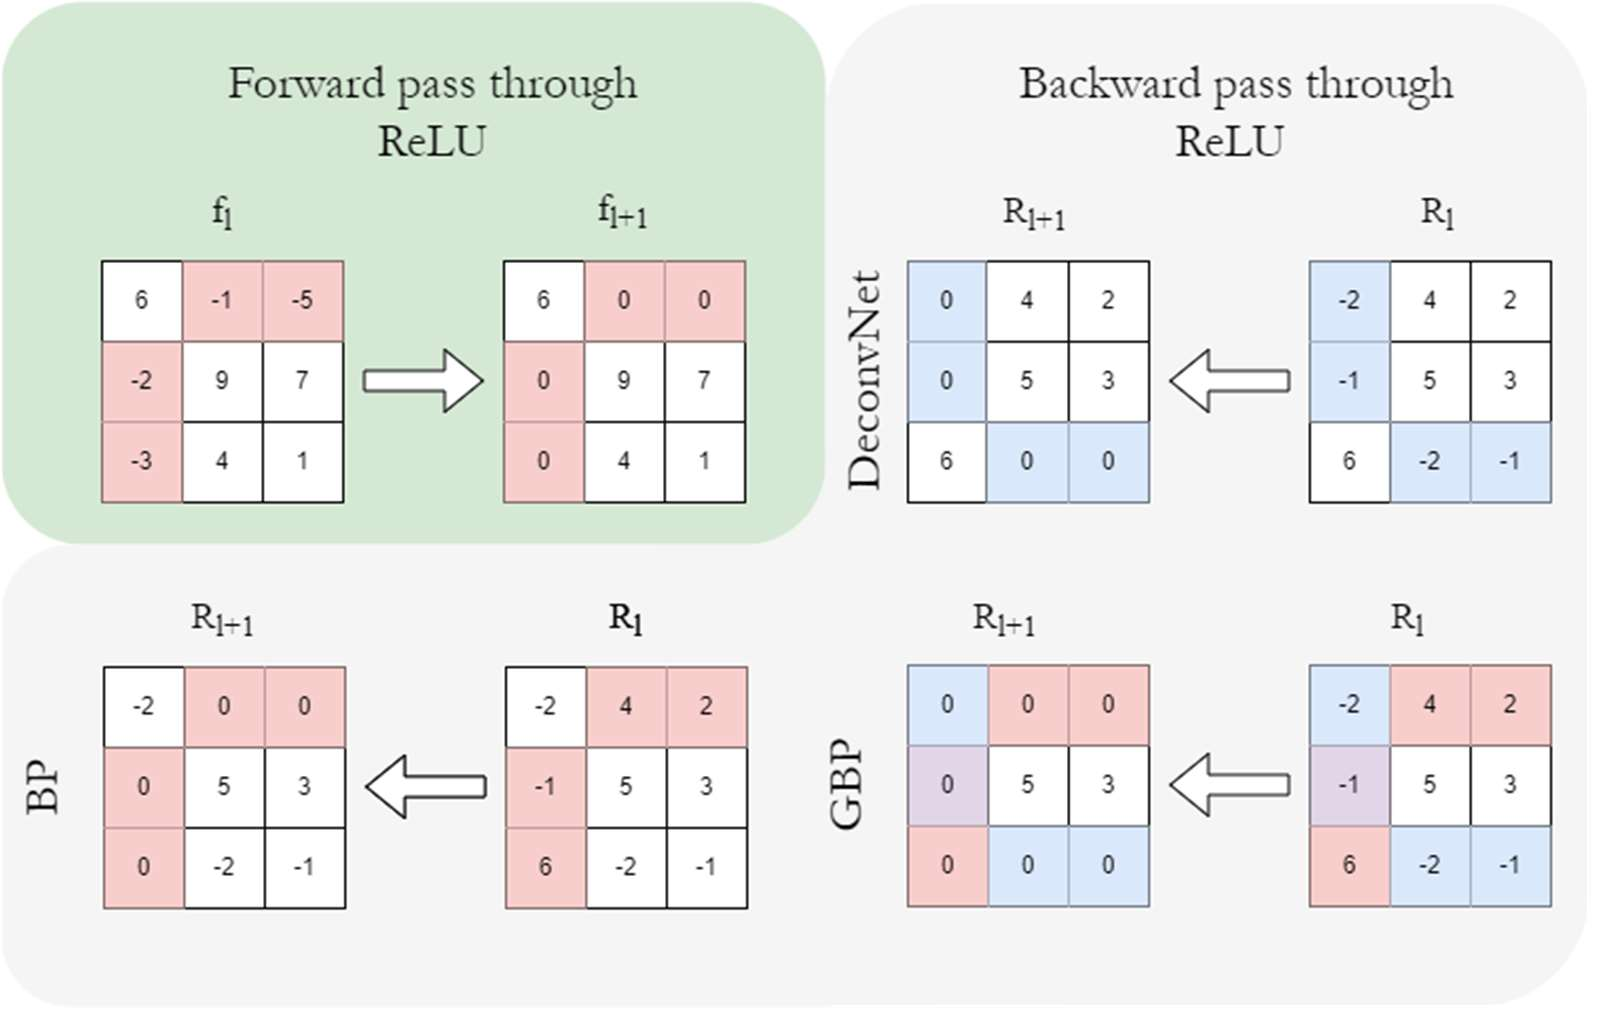
\includegraphics[width=\textwidth]{img/guided_backprop.png}
        \centering
    \end{figure}    
\end{minipage}
\hfill
\begin{minipage}{0.4\textwidth}
    \begin{itemize}
        \item Like DeconvNets, \textbf{only positive error signals are backpropagated} setting the negative gradients to zero.
        \item Like in Saliency, \textbf{only positive inputs are considered}. The advantage of retaining only positive gradients is to prevent a backward flow of negative contributions corresponding to neurons which inhibit the
        activation of the higher level neuron. As opposed to saliency, this can act as an additional guidance signal when traversing the network.
        \item The absolute value of the gradient is taken as the relevance score
    \end{itemize}
\end{minipage}

\subsubsection{SmoothGrad}
The idea of SmoothGrad by \cite{DBLP:journals/corr/SmilkovTKVW17} is to make gradient-based explanations less
noisy by adding noise and averaging over these artificially noisy gradients. SmoothGrad is not a standalone explanation method, but an extension to any gradient-based
explanation method.\\

SmoothGrad algorithm:
\begin{enumerate}
    \item Generate multiple versions of the image of interest by adding noise to it.
    \item Create pixel attribution maps for all images.
    \item Average the pixel attribution maps.
\end{enumerate}

The derivative fluctuates greatly at small scales. Neural networks have no incentive during training
to keep the gradients smooth, their goal is to classify images correctly. The solution is to average over multiple maps so as to “smooths out” these fluctuations.\\
\begin{equation*}
    A^c(x) = \frac{1}{N\_noise}\sum_{i-1}^{N\_noise} A^c(x+g_i)
\end{equation*}
Where $g_i\sim N(0, \sigma^2)$ are noise maps sampled from the Gaussian distribution.\\

Implementation suggestions: The ideal noise levels depends on the input image and the network. The authors suggest a level of 10-20\% which means $\frac{\sigma}{x_{max}-x_{min}}$ should be between 0.1 and 0.2.\\
$x_{max}$ and $x_{min}$ are the minimum and maximum pixel values of the image. The $N_{noise}$ is an hyperparameter which represents the number of generated noisy samples. The authors suggests $N_{noise}=50$

\subsubsection{Gradient $\odot$ input}
Proposed by \cite{DBLP:journals/corr/ShrikumarGSK16}. In Gradient $\odot$ input the attribution scores are calculated by elementwise multiplication of gradients with the input:
\begin{equation*}
    A^c(x) = |\frac{\partial S_c(x)}{\partial x}| \odot x
\end{equation*}
The element-wise multiplication can be considered as an application of a model-independent filter
(the input), which may reduce noise and smoothen the attribution map.

\subsubsection{Problem with gradients methods}
If $S_c(x)$ is flat in the proximity of $x_i$, $\frac{\partial S_c(x)}{\partial x_i}=0$ and so $x_i\frac{\partial S_c(x)}{\partial x_i}=0$ possibly erroneously indicating that feature $x_i$ is irrelevant.§
This happens because we train the model to saturation, thus the prediction score is near flat in the proximity of the input.\\

Thus, changing $x_i$ by a small amount $\partial x_i$ because the surface $\frac{\partial S_c(x)}{\partial x_i}$ is flat in that proximity it
will give us always zero — we are not looking at relevant gradients.\\

Therefore, to capture relevant gradients, some XAI methods have proposed to see how
gradients vary along a path from a reference neutral image (referred as the baseline) to the
feature value.

\subsection{Baseline attribution methods}
Compare the input image to a reference baseline image, which represent a neutral signal to the network.

This category includes model-specific gradient-based methods such as Deep Taylor andIntegrated Gradients, as well as model-agnostic methods such as LIME and SHAP.
The interpretation is always done with respect to the baseline: The difference between
classification scores of the actual image and the baseline image are attributed to the pixels.

The choice of the reference image (distribution) has a big effect on the explanation.

\subsubsection{Integrated Gradients}
Proposed by \cite{DBLP:conf/icml/SundararajanTY17}.
Let $x=\{x_i\}_{i=1}^N\in\mathbb{R}^N$ be the input and $x'=\{x'_i\}_{i=1}^N\in\mathbb{R}^N$ the baseline input. 
IG considers the straightline path in $\mathbb{R}^N$ from the baseline $x'$ to the input $x$, and compute the gradients at all points
along the path, accumulating them.\\

The IG along the ith dimension for an input $x$ and a baseline $x'$ is defined as:
\begin{equation*}
    IntegratedGrads_i(x) \Coloneqq (x_i-x'_i)\int_{\alpha=0}^1 \frac{\partial S_c(x'+\alpha(x-x'))}{\partial x_i}d\alpha
\end{equation*}
where $\frac{\partial S_c(x)}{\partial x_i}$ is the gradient of $S_c(x)$ along the $i^{th}$ dimension.\\

\textbf{Axioms}\\
\begin{itemize}
    \item \textit{Completeness}: the attributions for all input features should sum up to the difference between the output of the network at the given input and the output at a baseline input. Mathematically, this is expressed as: $\sum_{i=1}^N IntegratedGrads_i(x) = S_c(x)-S_c(x')$
    \item \textit{Sensitivity}: if an input feature changes while all other features remain constant and the change in the input feature causes a change in the model output, then the attribution for that input feature should be non-zero. Conversely, if the change in the input feature does not cause any change in the model output, the attribution should be zero.
    \item \textit{Implementation Invariance}: This axiom ensures that the attributions are consistent across functionally equivalent networks. If two networks compute the same function but are implemented differently (different architectures, parameterizations, etc.), the attributions should be the same.
    \item \textit{Linearity}: If the model's output is a linear combination of two functions, then the attributions should be the corresponding linear combination of the attributions for each function. Mathematically $S3_c(x)=a\cdot S1_c(x)+b\cdot S2_c(x)$ then \\$IntegratedGrads_c(x)=a\cdot IntegratedGrads1_c(x)+b\cdot IntegratedGrads2_c(x)$. Intuitively, the attributions preserve any linearity within the network.
    \item \textit{Symmetry}: For symmetric functions, symmetric inputs should have the same attributions. If the function $F(x, y) = F(y, x)$ , then the attributions for $x$ and $y$ should be equal.
\end{itemize}

\textbf{Graphical representation:}\\
\begin{figure}[H]
    \centering
    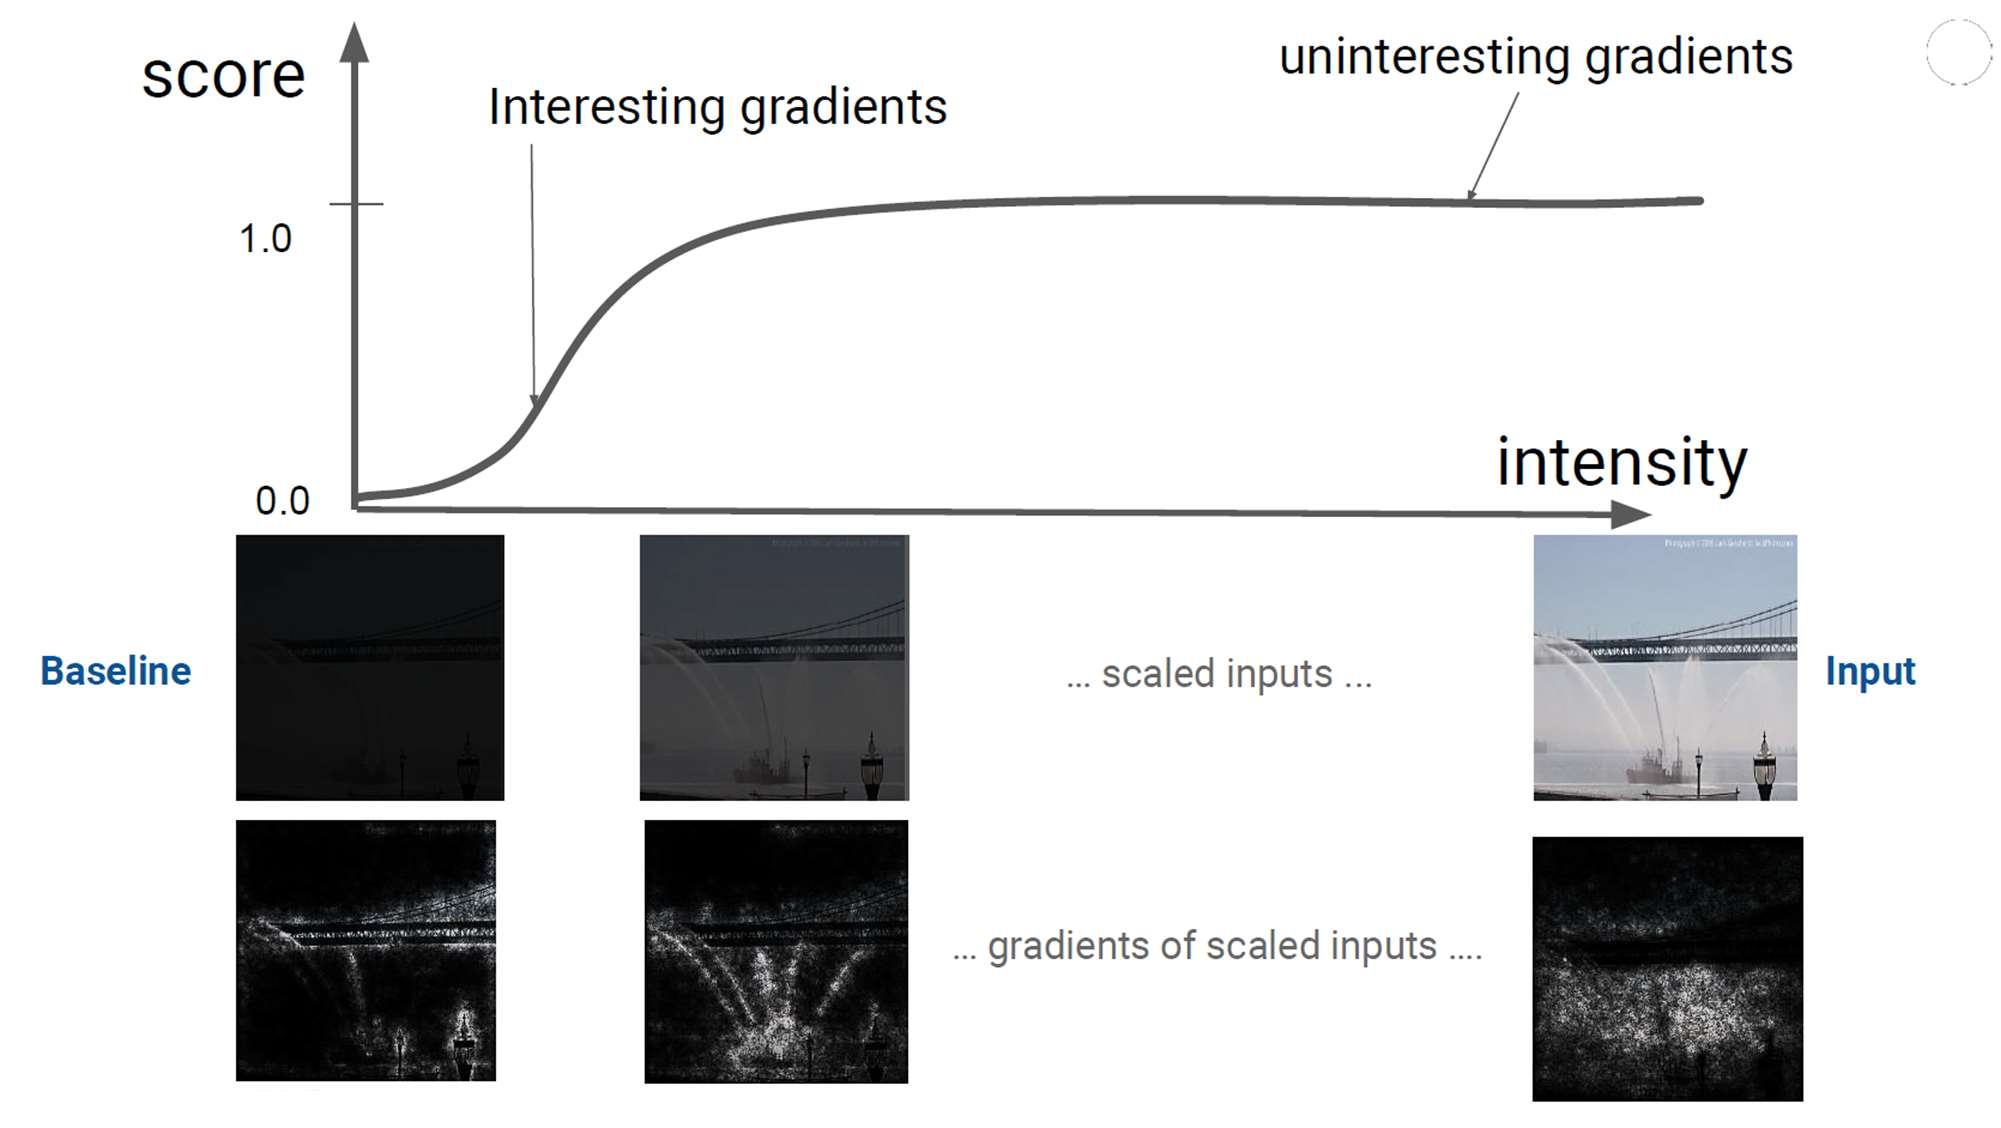
\includegraphics[width=0.7\textwidth]{img/IG.png}
\end{figure}

\textbf{Integrated Gradients vs Saliency maps}\\
\begin{minipage}{0.55\textwidth}
    \begin{figure}[H]
        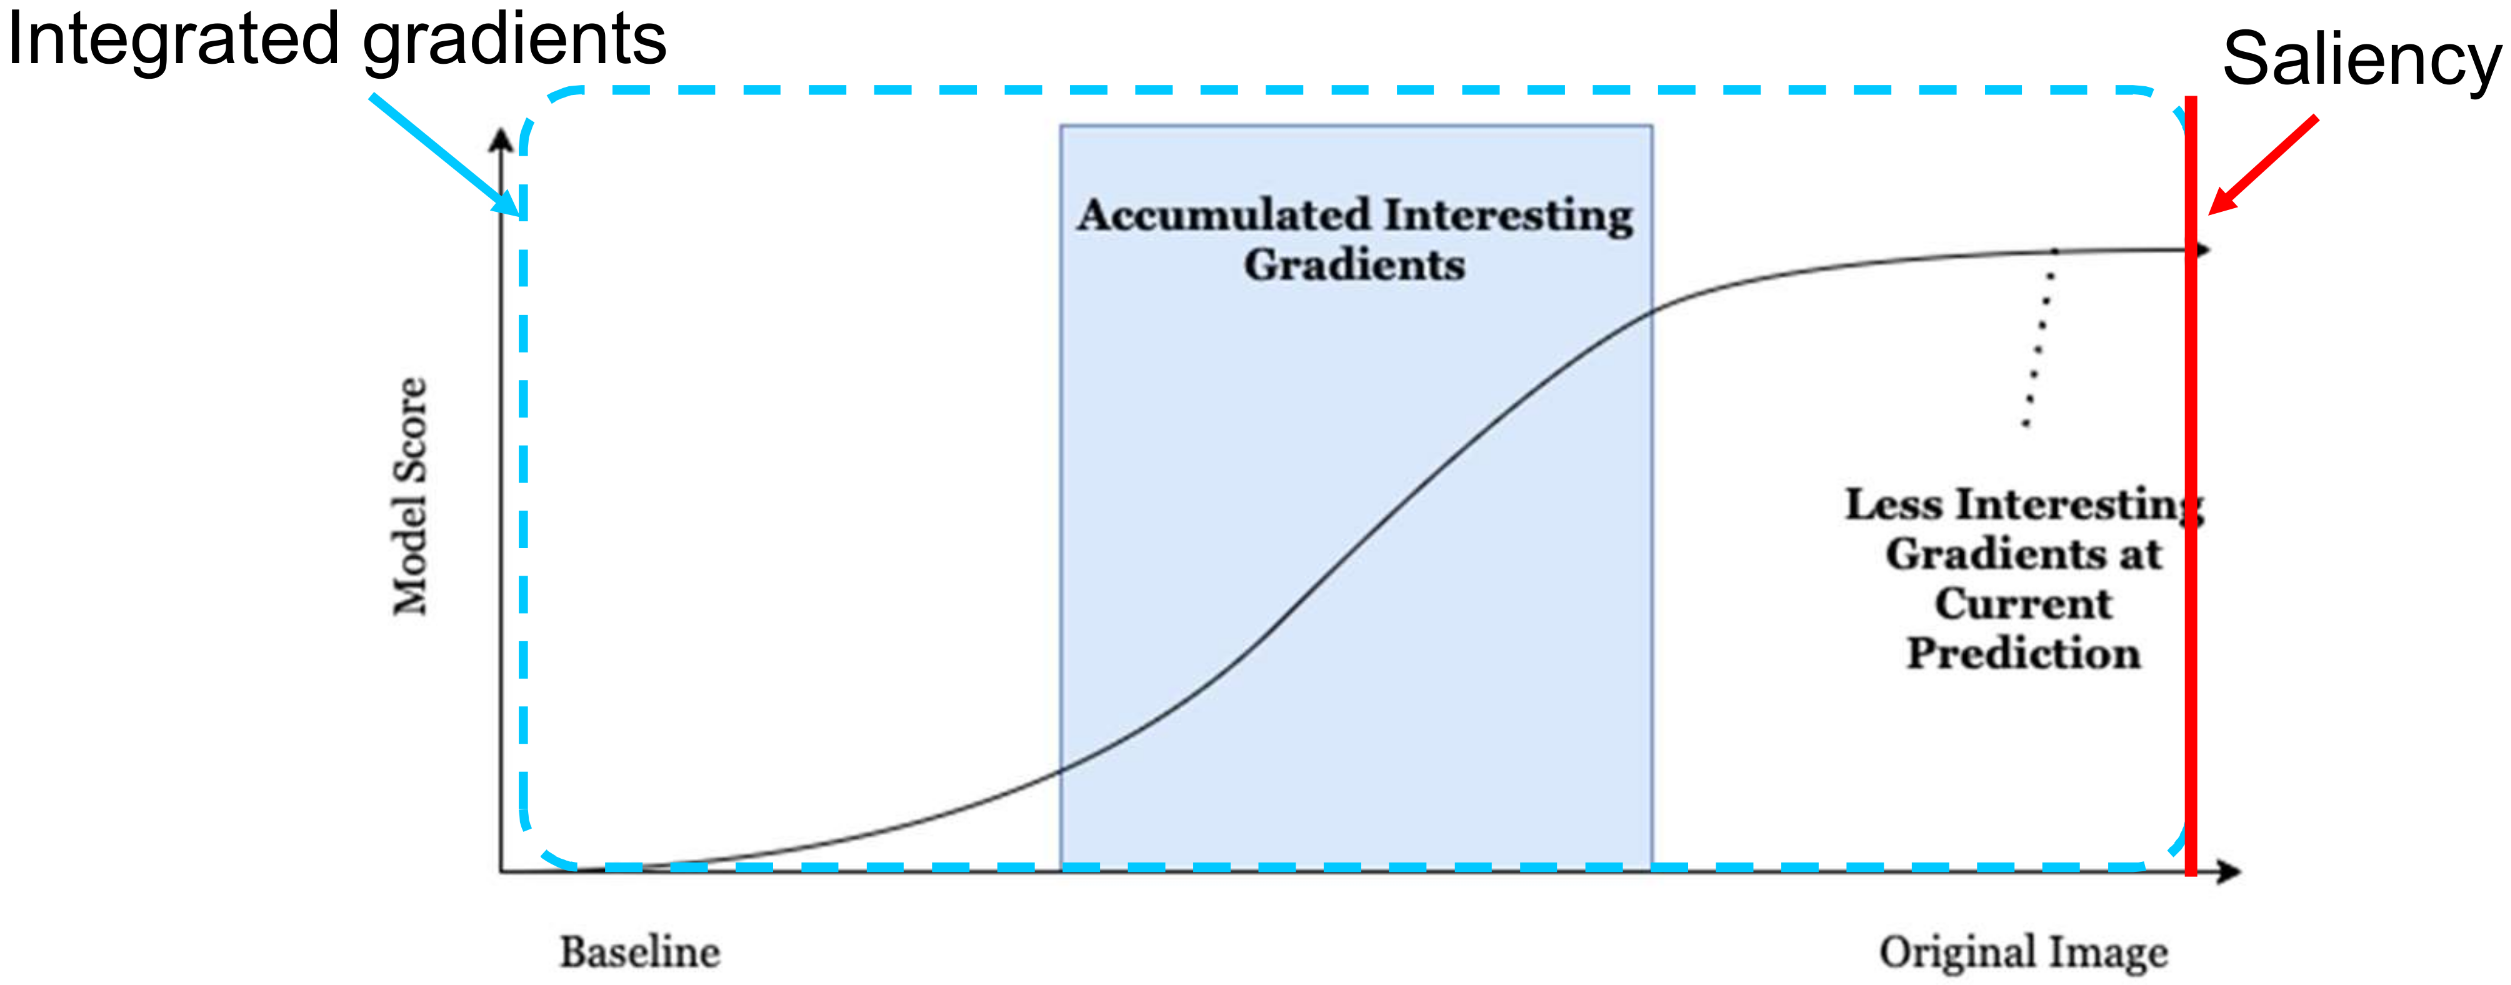
\includegraphics[width=\textwidth]{img/IGvsSM.png}
        \centering
    \end{figure}    
\end{minipage}
\hfill
\begin{minipage}{0.4\textwidth}
    As already seen, saliency maps are the gradients of the input features of a neural network with respect to
a final output. This explanation highlights the features that are the most reactive and likely to quickly
change the output, but only makes sense for small deviations away from the original input. Hence the
gradients received for saliency maps are generally in the model's saturated region of gradients.
\end{minipage}\\

\textbf{Practical implementation:}\\
The integral of integrated gradients can be efficiently approximated via a summation. We simply sum the gradients at points occurring at sufficiently small intervals along the straightline path from the baseline $x'$ to the input $x$.
\begin{equation*}
    IntegratedGrads_i^{approx}(x) \Coloneqq (x_i-x'_i)\sum_{k=1}^m \frac{\partial S_c(x'+\frac{k}{m}(x-x'))}{\partial x_i}\frac{1}{m}
\end{equation*}

Here $m$ is the number of steps in the Riemman approximation of the integral. Notice that the approximation simply involves computing the gradient in a for loop which should be straightforward and efficient in most deep learning frameworks.

The authors suggest that 20 and 300 steps are enough to approximate the integral (within 5\%) and recommend to check that the attributions approximately adds up to the difference between the score at
the input and that at the baseline, if not increase the step-size m.